\chapter{Expérimentations et Usages}
\section{Utilisation}
	Notre avons développé notre application avec du java standard Édition 11 pour des raisons compatibilité avec les ordinateurs de l'université. Elle peut s'exécuter sur les distributions Linux avec interface graphique tel que Ubuntu version 20.04.4 LTS, sur mac Os 12.3.1 et windows 10.
	
\section{Lancement de l'application}
 	Vous devez ouvrir un terminal à l'emplacement du dossier .
 	\\ \\
 	Pour :
 	\begin{itemize}
 		\item Lancer l'application exécuter : \fbox{ \textbf{\em ant run}} ou \fbox{ \textbf{\em ./scripts/run.sh}}
 		\item Initialiser le projet: \fbox{\textbf{\em ant init}}  ou fbox{\textbf{\em ./scripts/install.sh}} \\
 			Cette initialisation créera  les dossiers de bases  bin, doc et dist 
 		\item Compiler le projet: \fbox{\textbf{\em ant compile}} ou \fbox{\textbf{\em ./scripts/compile.sh}}
 		\item Générer le Javadoc: \fbox{\textbf{\em ant javadoc}} ou \fbox{\textbf{./scripts/makedoc.sh}}		
 		\item Générer le fichier jar: \fbox{\textbf{\em ant packaging}} ou \fbox{\textbf{\em ./scripts/makejar.sh}}
 		\item Exécuter le fichier jar:\fbox{\textbf{\em ./scripts/	runjar.sh}}
 		\item Nettoyer le projet: \fbox{\textbf{\em ant clean}} ou \fbox{\textbf{\em ./scripts/clean.sh}}
 		\item Lancer le test: \fbox{\textbf{\em ant test}} ou \fbox{\textbf{\em ./scripts/test.sh}}
	\end{itemize} 		
 	
\section{Fonctionnement de l'interface Graphique}
	Au lancement du programme, il se présente avec un exemple par défaut visualisable  
par clic sur le bouton \textbf{Generate} sous forme 2D ou 3D.\\
	Dans la barre de menu existe une liste déroulante contenant d'autres exemples ainsi qu'un bouton aide permettant à l'utilisateur de mieux comprendre le fonctionnement de l'interface et l'interprétation des symboles.

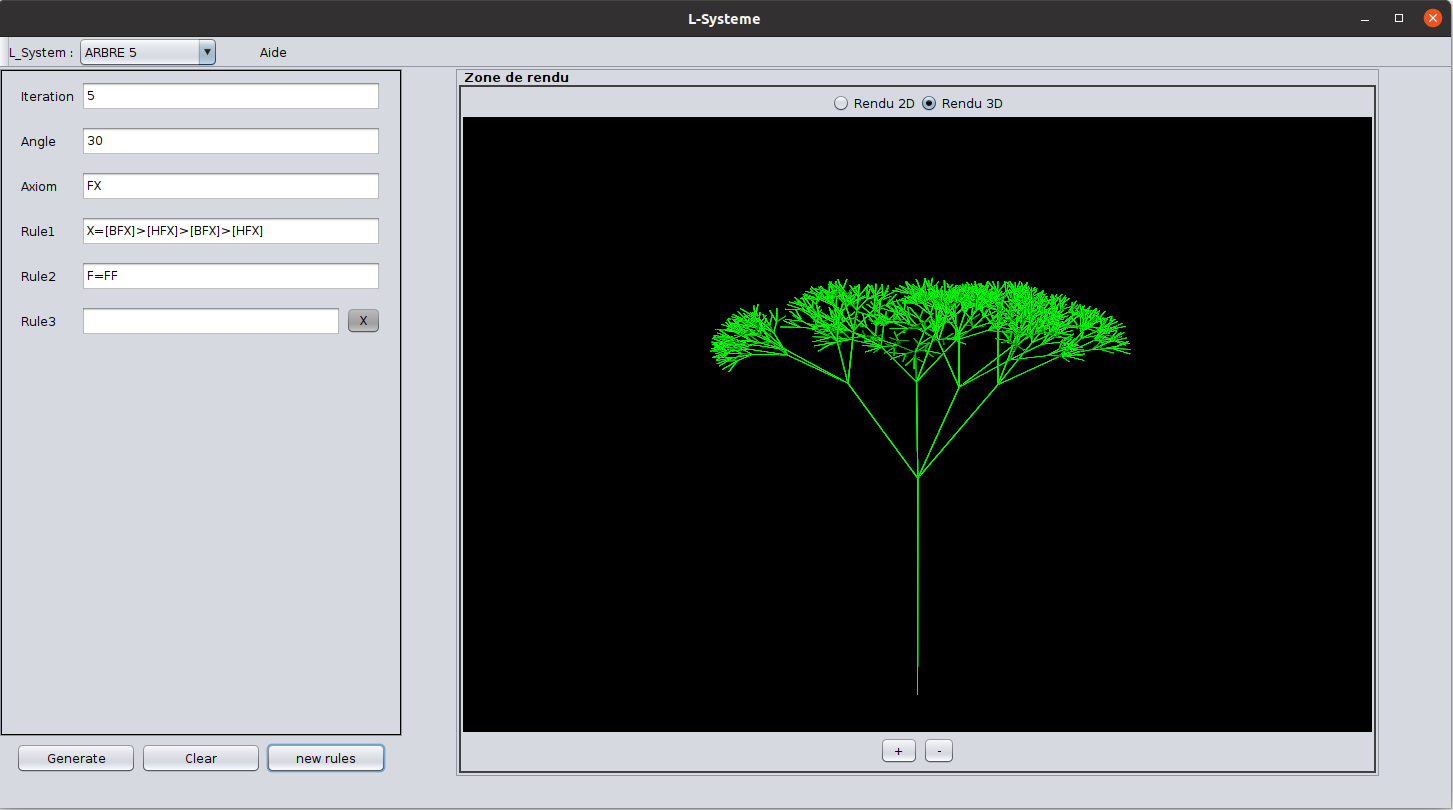
\includegraphics[width=16cm]{images/interface.png}
\\
\\
Il est possible qu'un utilisateur puisse composer ses  propres règles. Pour cela les boutons \textbf{ clear, Generate} et \textbf{Newrule} lui sera d'une aide (voir Configuration~\ref{config} page \pageref{config}) pour l'utilisation des ces boutons.

Attention  l'application tient compte de la caste. Toute modification entraînée sur l'interface graphique il faudrait cliquez sur le bouton \textbf{Generate} pour la visualiser.

Dans la zone rendu  à gauche le rendu 2d est coché par défaut est vous pouvez le remettre sur le rendu 3D. 

%En 3D des éléments supplémentaires sont ajoutées aux règles .
\section{Navigation dans l'interface graphique 3D}

Pour naviguer dans l'espace 3D les boutons : + ou - serviraient à zoomer  ou dézoomer respectivement.
\\
\begin{itemize}
	\item Bouton \textbf{+} permet de zoomer
	\item Bouton \textbf{-}  permet de dézoomer 
\end{itemize}

En plus un clic glissé de la souris :
\begin{itemize}
	\item Vers la droite : permet de faire tourner l'arbre autour de lui même dans la même direction;
	\item Vers la gauche: permet de faire tourner l'arbre  autour de lui même dans la même direction ;
	\item Vers le bas: incline l'arbre vers le bas 
\end{itemize}
\newpage
\section{Test du logiciel}
\subsection{Possible problème}
	Lorsque vous lancer et essayer de générer un arbre avec un nombre d'itération au delà d'un certain seuil suivant la composition de l'arbre, cela pourrait prendre un peu de temps pour le parseur lors de la réécriture et sa représentation 3D voir 2D pourrait déborder. Dans ce cas une solution serait de diminuer le nombre d'itération, en plus en 3D on pourrait aussi dézoomer.

\subsection{Test du logiciel}
	Nous avons réalisé nos tests en utilisant le framework open source \textbf{Junit-4.12} le développement et l'exécution de tests unitaires. Elle teste l'ensemble des méthodes indispensables pour la réécriture d'un arbre.
\\ 
	\begin{figure}[h]
		\centering
		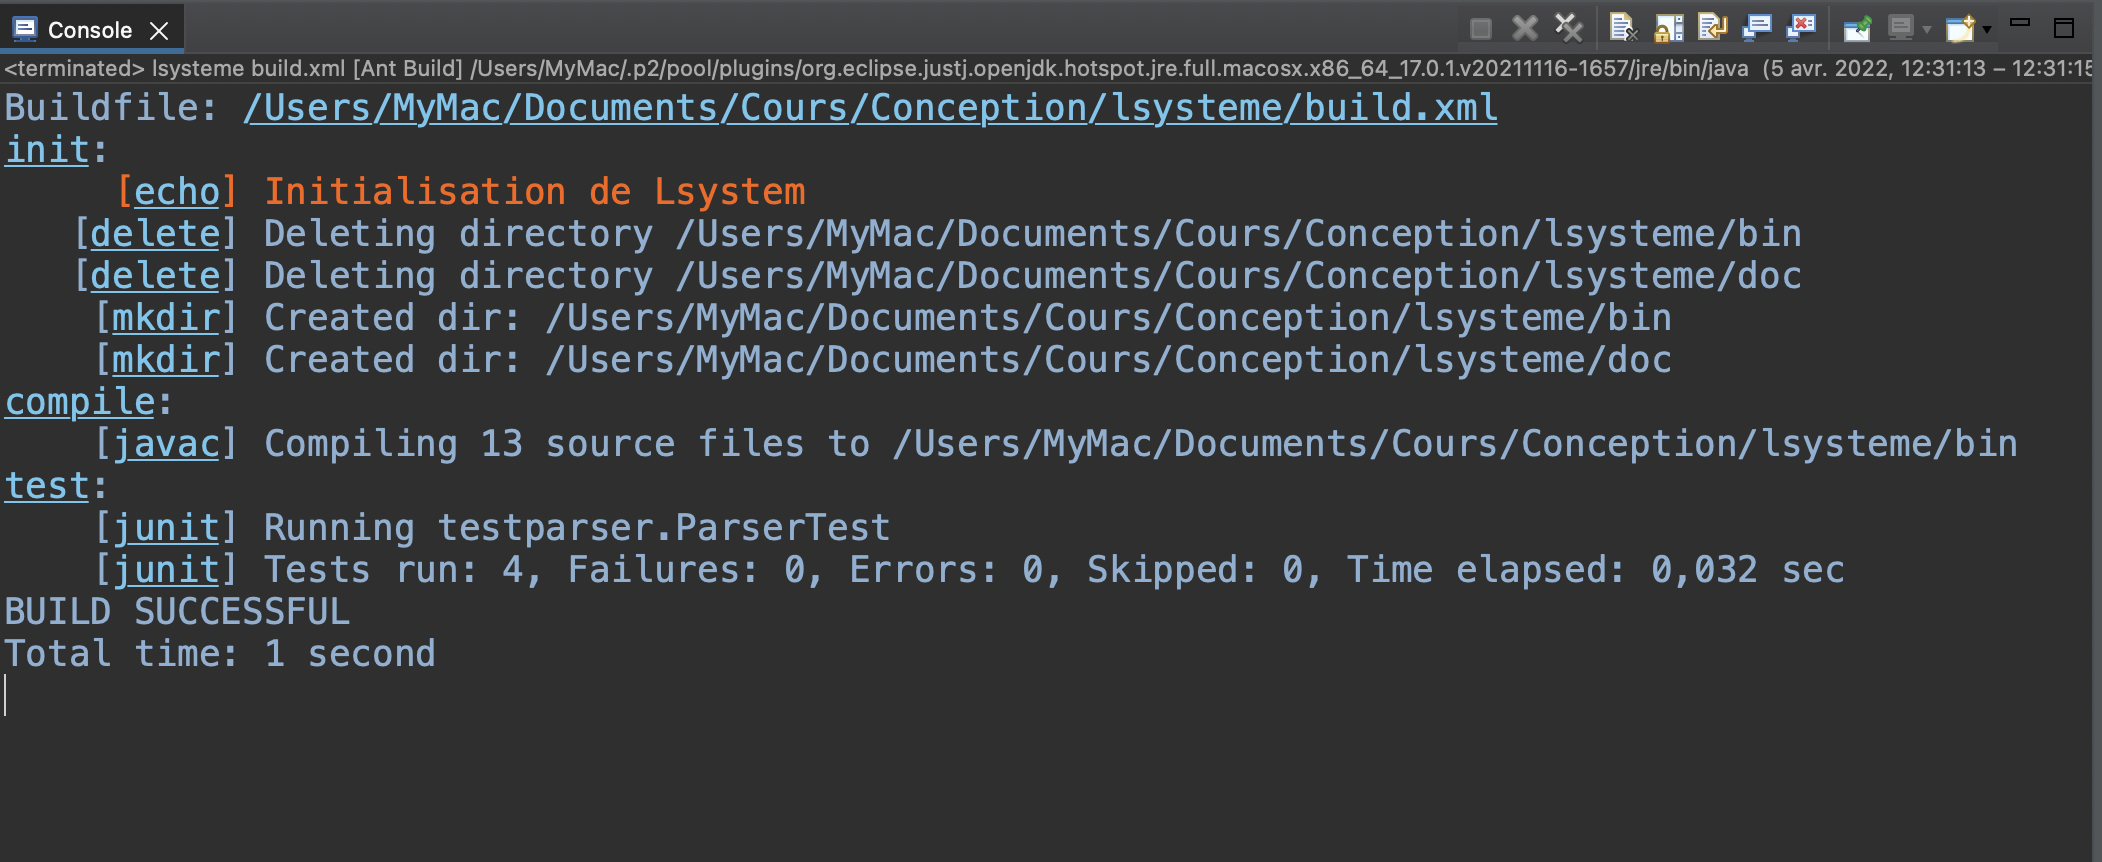
\includegraphics[width=16cm]{images/test.png}
	    \caption{Test }
	\end{figure}